\section{Hardware Specification \& Wiring}
\label{sec:hardware_design}

\begin{figure}[H]
    \centering
    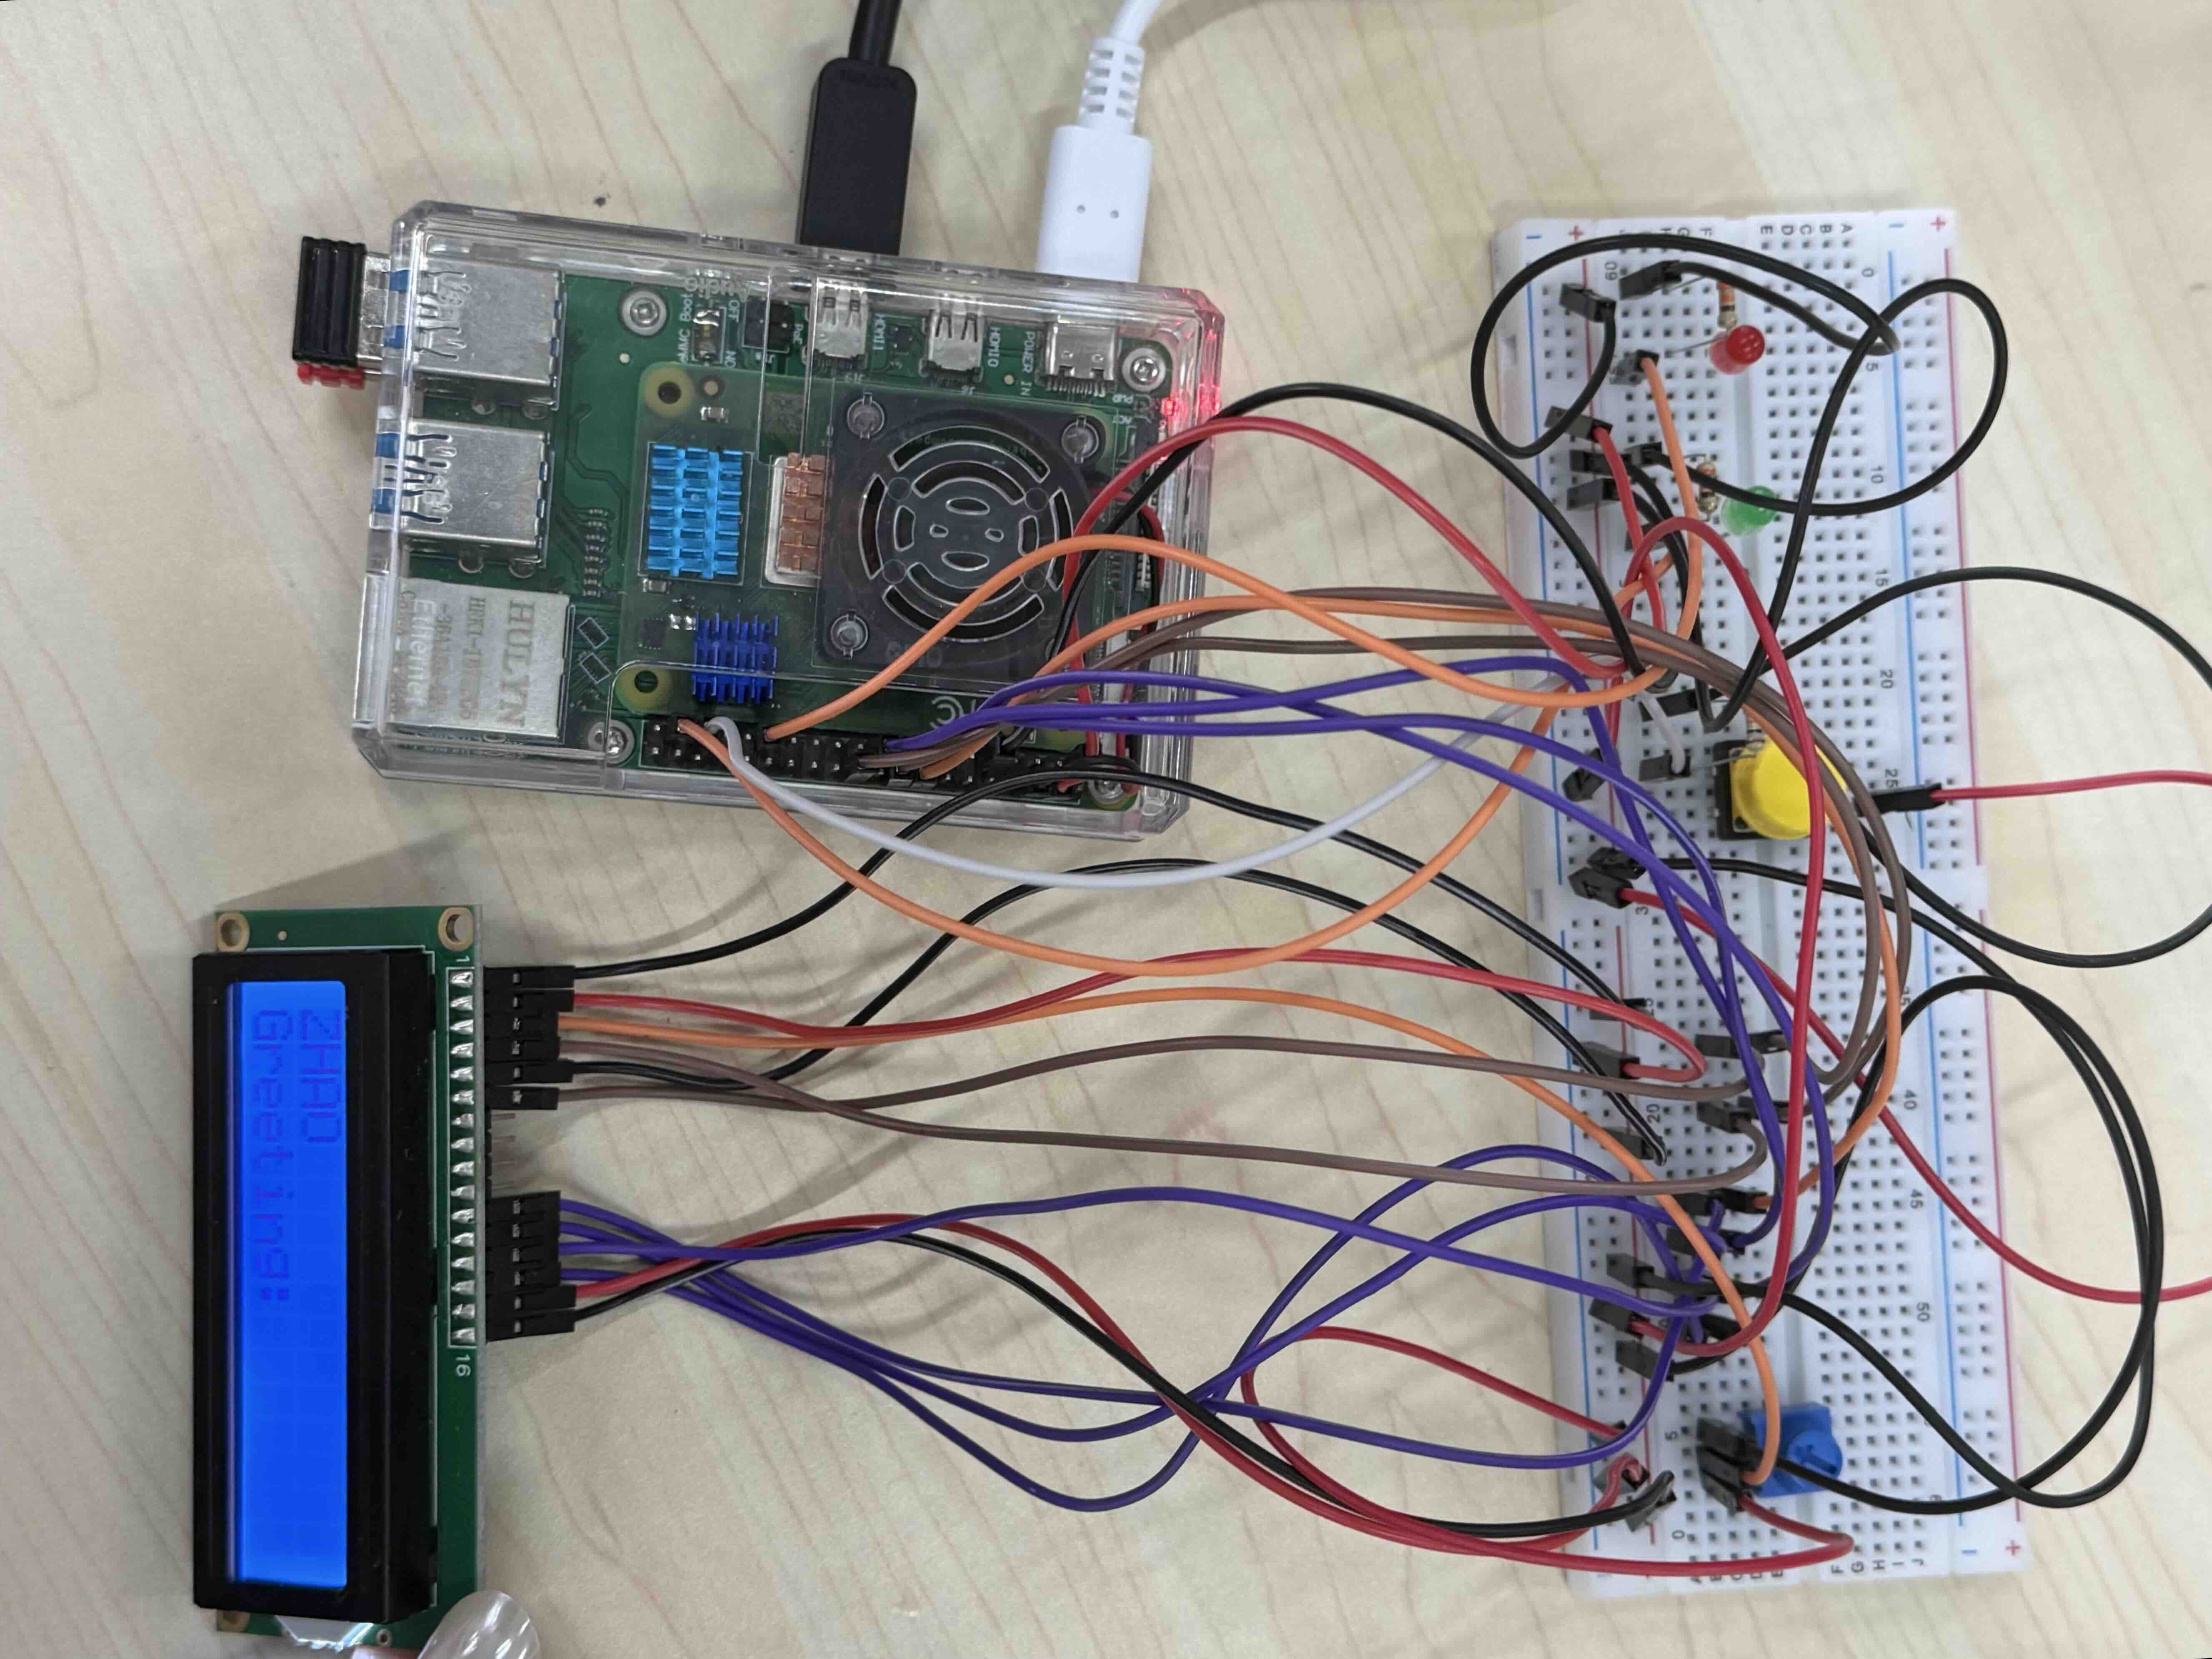
\includegraphics[width=0.8\columnwidth]{figures/hardware_wiring.jpg} 
    \caption{Schematic diagram of physical wiring.}
    \label{fig:wiring}
\end{figure}

The hardware platform of this project is Raspberry Pi, which runs a 32-bit system to ensure the compatibility of ARM assembly instructions. The external physical interaction system consists of several basic electronic components, including leds (red and green) for visual feedback, physical buttons for receiving user input, and an LCD display for displaying text information. In addition, a sliding rheostat is connected to dynamically adjust the contrast of the LCD display to ensure the visibility of the output information.

\vspace{-1em}

\begin{table}[H]
    \centering
    \caption{LED \& Button Configuration}
    \label{tab:led_button_config}
    \begin{tabularx}{\columnwidth}{@{}l l X@{}}
        \toprule
        \textbf{Modules} & \textbf{GPIO Pin} & \textbf{Function} \\
        \midrule
        Green LED   & GPIO 26   & Repeat user input and indicate successful search results. \\
        Red LED     & GPIO 5    & Status separation and input acknowledgment. \\
        Button      & GPIO 19   & Record the PIN sequence through timed presses. \\
        \bottomrule
    \end{tabularx}
\end{table}

\vspace{-1em}

All components are connected to the GPIO pins of the Raspberry Pi through the breadboard. The green led for data echo indication is connected to the GPIO 26 pin through a series 330$\omega$ resistor, and the red led for control signal and status separation is connected to the GPIO 5 pin. The physical button is plugged into a GPIO 19 pin and is configured in input mode in the system software for high-frequency polling to capture the user's actions.

\vspace{-1em}

\begin{table}[H]
    \centering
    \caption{LCD Display Configuration}
    \label{tab:lcd_config}
    \begin{tabularx}{0.75\columnwidth}{@{}l l X@{}}
        \toprule
        \textbf{LCD Pin} & \textbf{GPIO Pin} & \textbf{Function} \\
        \midrule
        1  (VSS)    & GND           & Ground                \\
        2  (VDD)    & 3V3           & Power Supply          \\
        3  (V0)     & Potentiometer & Contrast Adjustment   \\
        4  (RS)     & GPIO 25       & Register Select       \\
        5  (RW)     & GND           & Read / Write Control  \\
        6  (EN)     & GPIO 24       & Enable                \\
        11 (D4)     & GPIO 23       & Data Bit 4            \\
        12 (D5)     & GPIO 10       & Data Bit 5            \\
        13 (D6)     & GPIO 27       & Data Bit 6            \\
        14 (D7)     & GPIO 22       & Data Bit 7            \\
        15 (LED+)   & 3V3           & Backlight Anode       \\
        16 (LED-)   & GND           & Backlight Cathode     \\ 
        \bottomrule
    \end{tabularx}
\end{table}

\vspace{-1em}

For the most complex LCD display, we use 4-bits data transmission mode for wiring. The logic power supply (pin 2) and backlight power supply (pin 15) of LCD are connected to the 3v3 power supply of Raspberry Pi, and the ground pins (pin 1, 5, 16) are connected to the GND. The register select pin RS (pin 4) is connected to GPIO 25, the enable pin EN (pin 6) is connected to GPIO 24, and the read / write pin RW is directly grounded to lock the screen into write mode. LCD 4-bit data pins D4-D7 (pin 11-14) connect GPIO 23, 10, 27, and 22 of Raspberry Pi in turn, thus forming a complete and reliable underlying data transmission bus.
